\section{Detectors}
\label{Sect:Detectors}

In this section, the resolution and efficiency of the detector systems is
discussed. The reconstruction is validated both internally within each
detector system, using the detector's internal redundancy, and by extrapolating
reconstructed events between detectors.

\subsection{Tracker}

Two trackers, made up of five stations each with three planes of scintillating
fibres are used to reconstruct the momentum of incoming particles. Particles 
make helical trajectories whose radius and wavelength vary according to the
transverse and longitudinal momentum respectively. The radius of the helix is
given approximately by
\begin{equation}
\label{eq:scifi_helix_radius}
r = \frac{p_t}{q B_z}
\end{equation}
and the wavenumber by
\begin{equation}
\label{eq:scifi_helix_wavenumber}
k = \frac{q B_z}{p_z}.
\end{equation}

Fitting is performed in several steps. Electronics signals arising from adjacent
fibres are collected into clusters. The position of clusters in adjacent planes 
are collected to form a space point. A first-pass fit of a perfect helix to the 
space points, pattern recognition, is used for noise rejection and to seed a 
second-pass fit using a Kalman filter. Tracks that do not fit a helix but 
successfully fit a straight line are seeded using the time-of-flight between
ToF0 and ToF1 to estimate momentum.

The trackers are the main detectors used in this analysis. The efficacy of the
trackers is discussed below.

\subsubsection{Resolution}

\begin{figure}[!tbh]
    \centering
    \includegraphics*[width=0.45\textwidth]{03-Detectors/Figures/hall-probes_2017-02-7/hp_65.pdf}
    \includegraphics*[width=0.45\textwidth]{03-Detectors/Figures/hall-probes_2017-02-7/hp_77.pdf}
    \includegraphics*[width=0.45\textwidth]{03-Detectors/Figures/hall-probes_2017-02-7/hp_79.pdf}
    \includegraphics*[width=0.45\textwidth]{03-Detectors/Figures/hall-probes_2017-02-7/hp_67.pdf}
    \includegraphics*[width=0.45\textwidth]{03-Detectors/Figures/hall-probes_2017-02-7/hp_66.pdf}
    \includegraphics*[width=0.45\textwidth]{03-Detectors/Figures/hall-probes_2017-02-7/hp_72.pdf}
    \caption{Hall probe readings for the four datasets across the entire period 
             where data was taken.\label{fig:hall_probes}}
\end{figure}

In the first instance, the correct operation of the tracker is studied by
examining the quality of the fitted tracks and comparing the measured magnetic 
field with the field assumed during reconstruction.

If the reconstruction is well-understood, the path of the reconstructed 
trajectories should match the position of the clusters. The $\chi^2$ distribution
per degree of freedom of reconstructed tracks was shown in fig. 
\ref{fig:tku_chi2} and \ref{fig:tkd_chi2} for the upstream and downstream
detectors respectively.

In order to accurately reconstruct tracks the field must be well known. If the
modelled field used in reconstruction differs from the actual field, a helix
can be found but the reconstructed longitudinal and transverse momenta will 
scale with the field according to eq. (\ref{eq:scifi_helix_radius}) and eq. 
(\ref{eq:scifi_helix_wavenumber}). In order to accurately reconstruct the field 
correctly it is essential to understand the field accurately in the measurement
region.

\begin{figure}[!tbh]
    \centering
    \includegraphics*[width=0.45\textwidth]{03-Detectors/Figures/field_2017-02-7/bfield_vs_z_ssu}
    \includegraphics*[width=0.45\textwidth]{03-Detectors/Figures/field_2017-02-7/bfield_vs_z_ssd}
    \caption{Hall probe readings compared to the field model used for 
             reconstruction and track extrapolation. Blue dashed lines show the
             position of the tracker stations.\label{fig:field_map}}
\end{figure}

\begin{table}
\caption{The ``as designed'' axial and azimuthal position of hall probes is listed.
\label{tab:hp_position}}
\centering
\begin{tabular}[pos]{l|rr}
Hall Probe & Axial position [mm] & Azimuthal position [ $^{\circ}$]\\
\hline
SSU HP 77 & 14104 & 30 \\
SSU HP 79 & 14429 & 270 \\
SSU HP 65 & 14429 & 30 \\
SSU HP 67 & 15286 & 150 \\
\hline
SSD HP 66 & 18625 & 210 \\
SSD HP 72 & 19482 & 330 \\
\end{tabular}
\end{table}

The field in the tracker region was monitored during the data taking period by
several Hall probes. The Hall probe measurement in the tracker region is shown
in fig. \ref{fig:hall_probes} for the data taking
periods under study in this paper. Reproducibility is demonstrated at around the
$10^{-3}$ T level for HP67 and around $10^{-4}$ T level for the other hall probes.
The design position of the Hall probes is listed in table \ref{tab:hp_position}. HP67 
and HP66 were both dislocated from their design position
during installation and so the actual position is uncertain. They are included 
here for reference only.

The measured fields are shown overlayed with the modelled field in the tracker 
region in fig. \ref{fig:field_map}. The SSU and SSD coil currents have been 
tuned so that the modelled field agrees with the measured field, and this tuned 
field is used for simulation and reconstruction.

The simulated resolutions for TKU and TKD are shown in fig. \ref{fig:tku_resolution}
and \ref{fig:tkd_resolution} respectively. A small systematic bias is noted in 
the momentum reconstruction. The asymmetry can arise due to the intrinsic angular momentum
of the beam or a simulated misalignment of the detector and field. 
Significant tails are apparent in the $p_z$ residual. Low transverse 
momentum tracks are challenging to reconstruct. The tails are longer
in TKD, where the field is 2 T rather than 3 T as in TKU.

\begin{figure}[!tbh]
    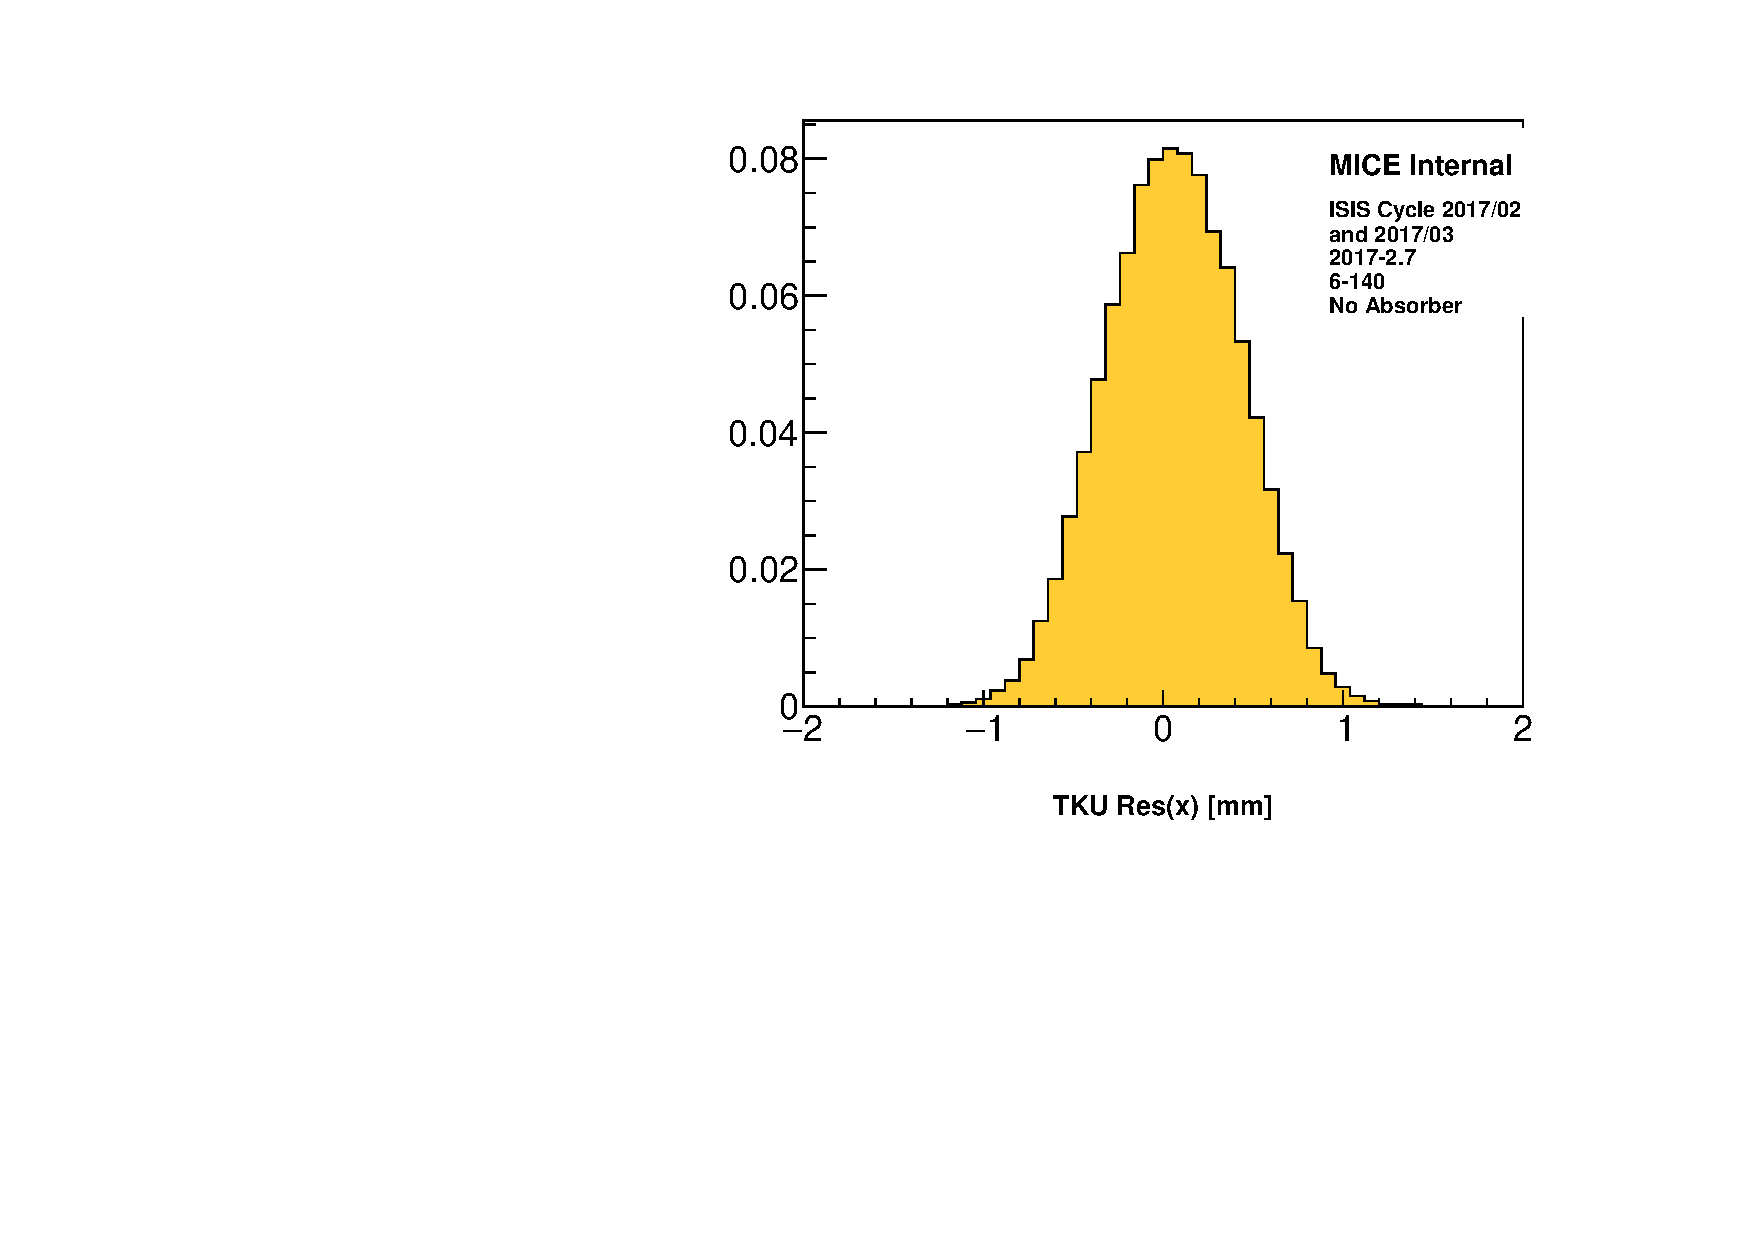
\includegraphics[width=0.5\textwidth]{03-Detectors/Figures/compare_mc/2017-2.7_6-140_None/tku_x}
    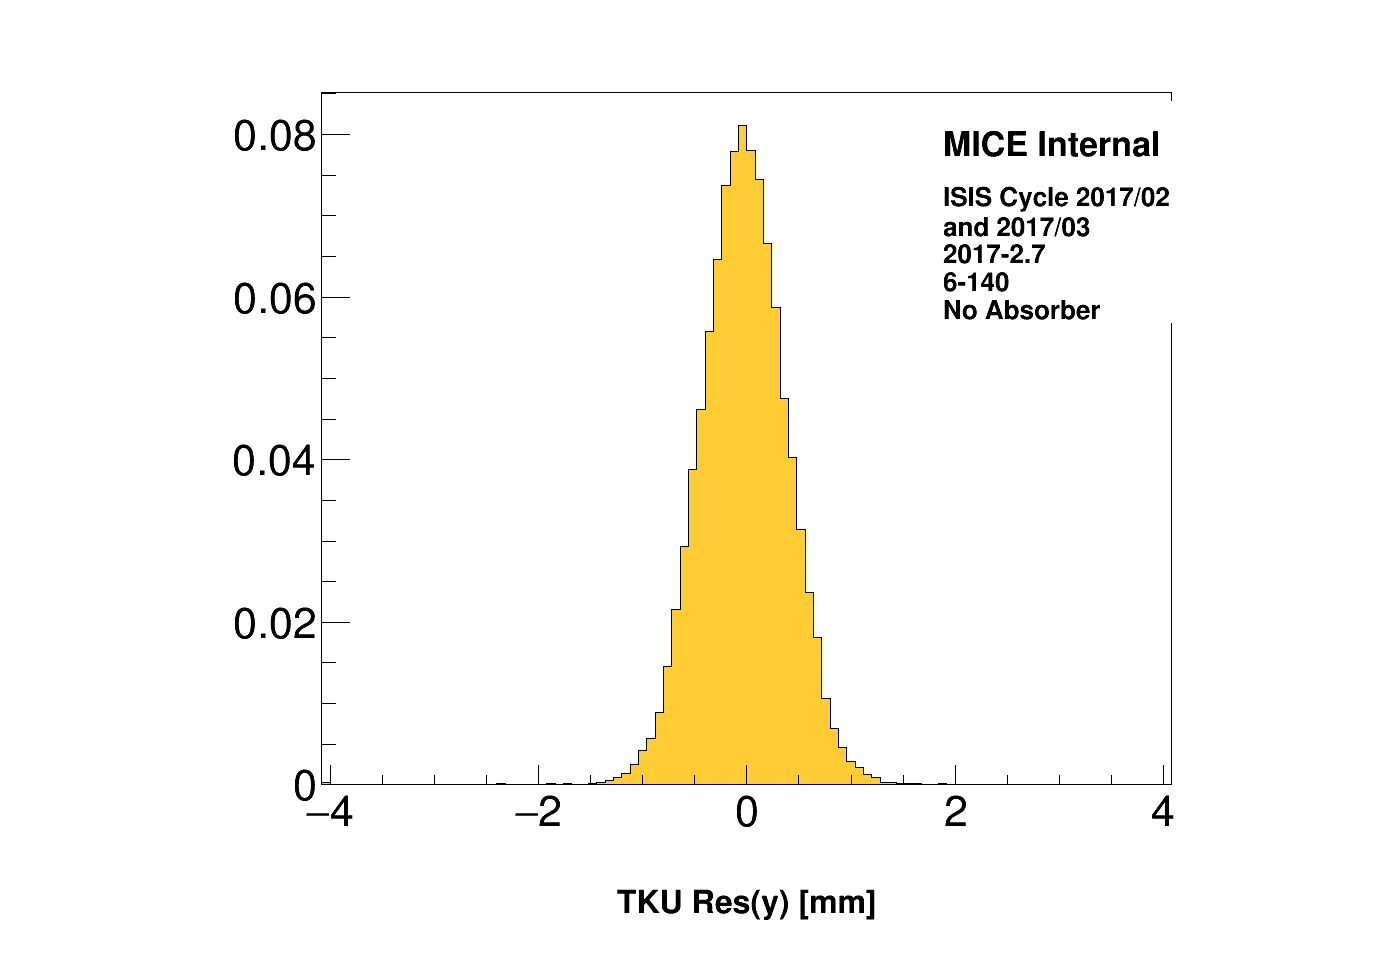
\includegraphics[width=0.5\textwidth]{03-Detectors/Figures/compare_mc/2017-2.7_6-140_None/tku_y}
    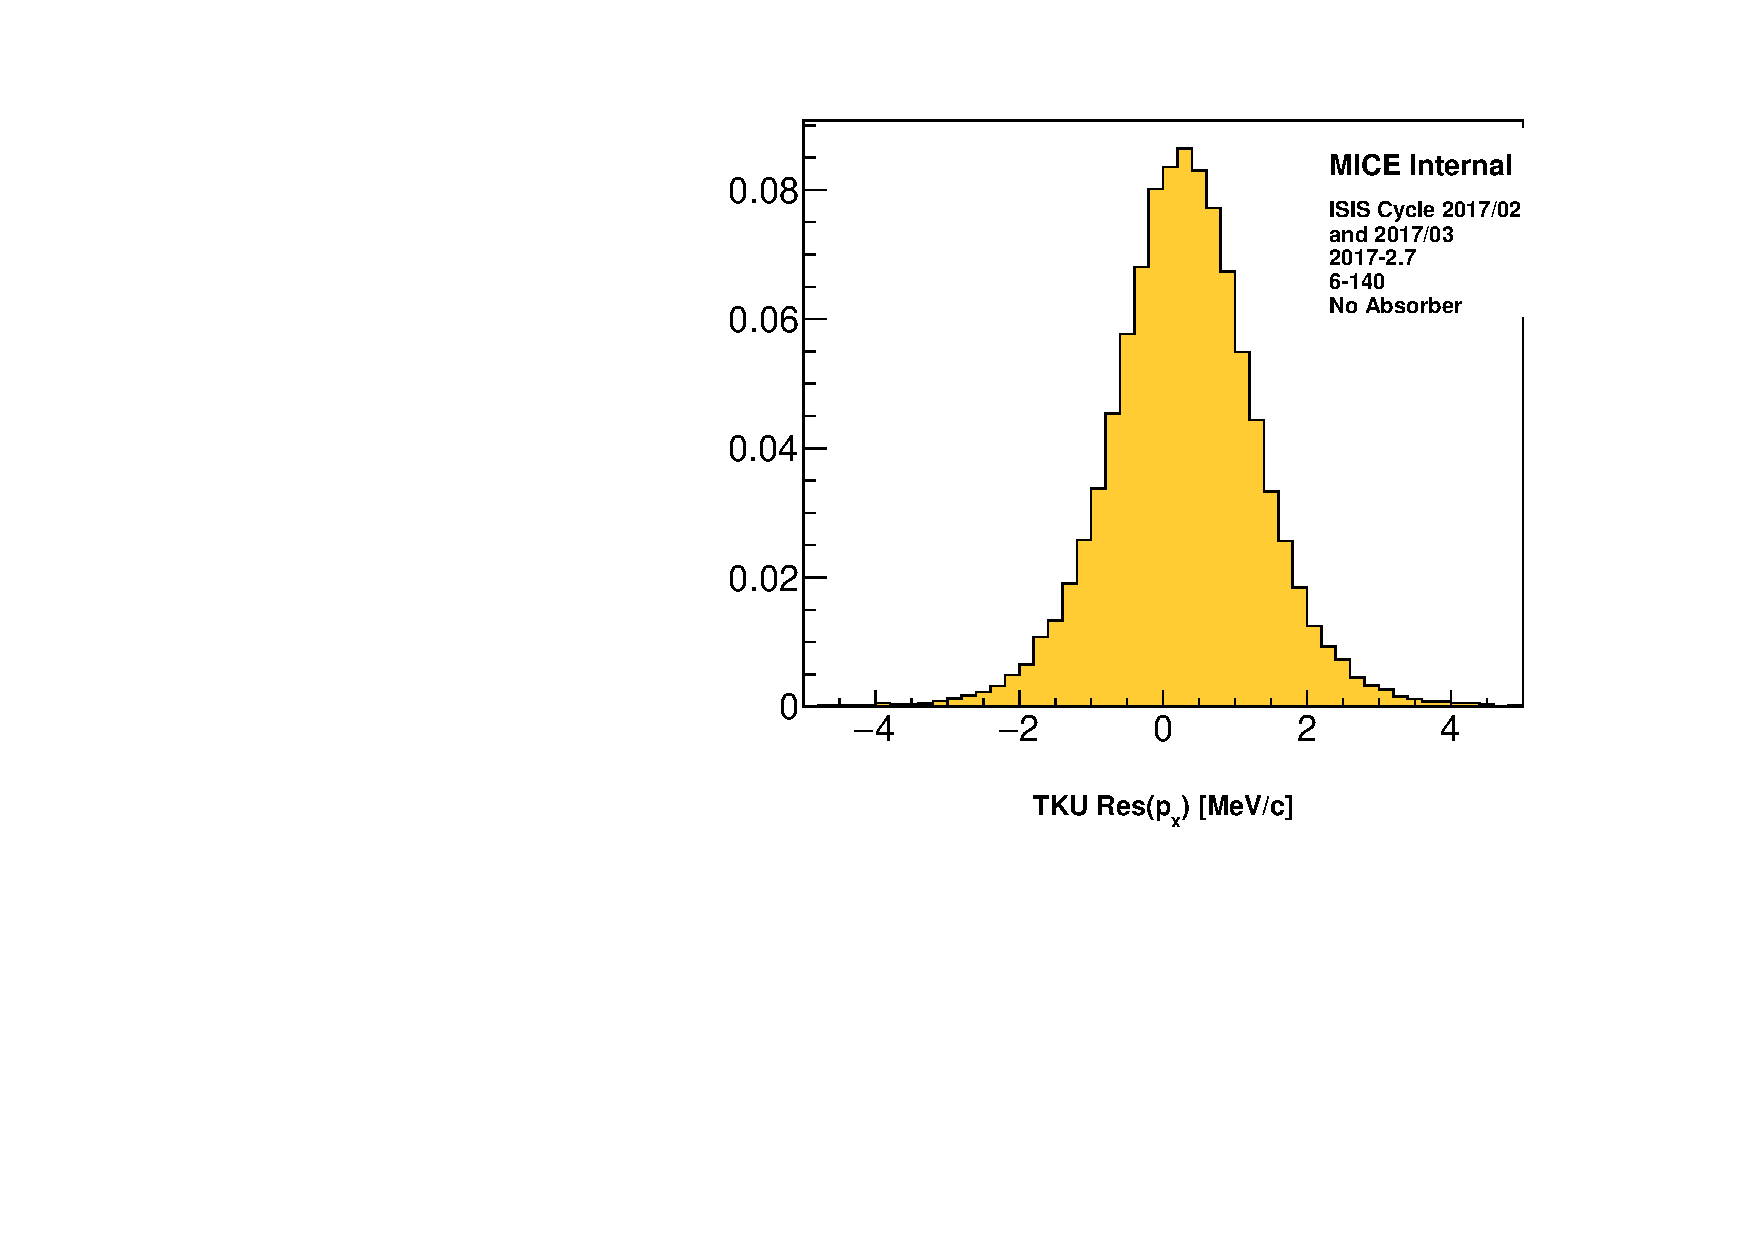
\includegraphics[width=0.5\textwidth]{03-Detectors/Figures/compare_mc/2017-2.7_6-140_None/tku_px}
    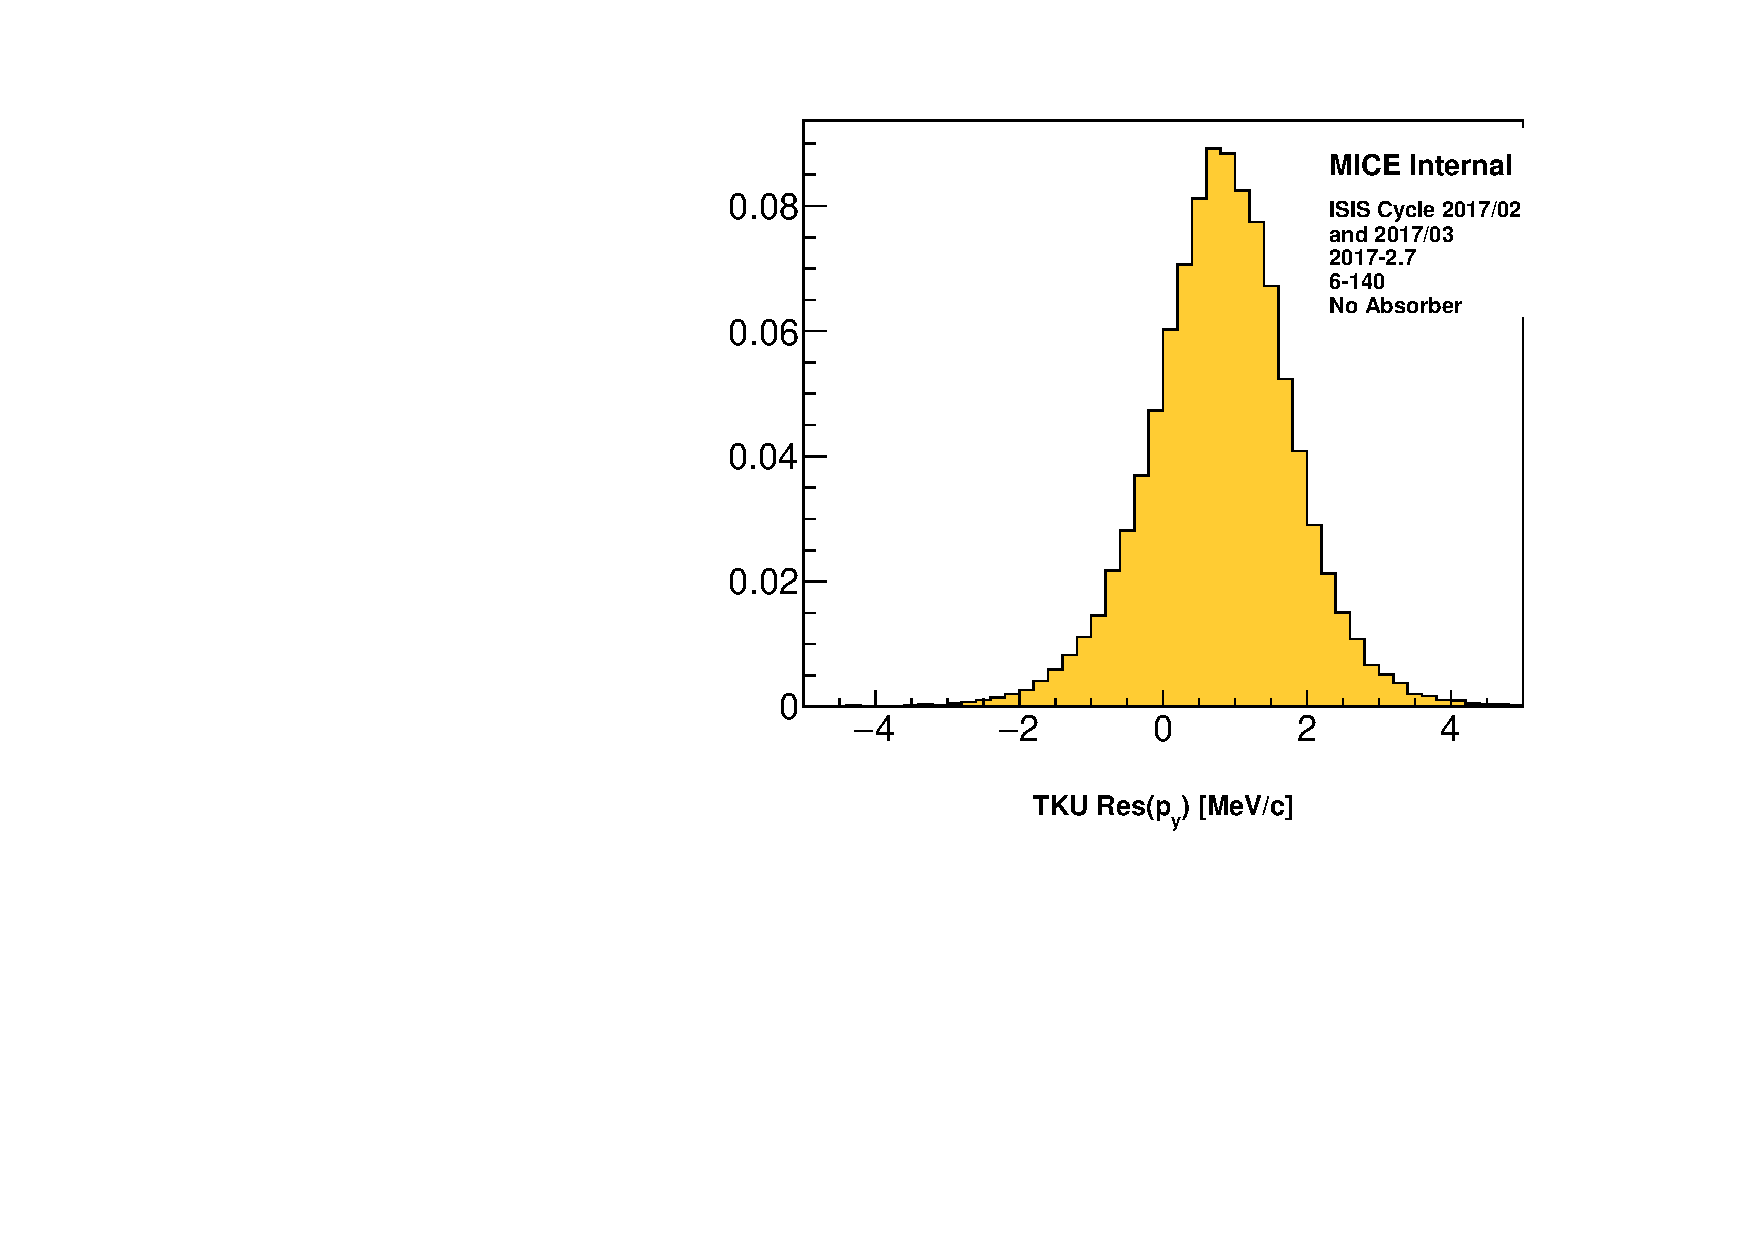
\includegraphics[width=0.5\textwidth]{03-Detectors/Figures/compare_mc/2017-2.7_6-140_None/tku_py}
    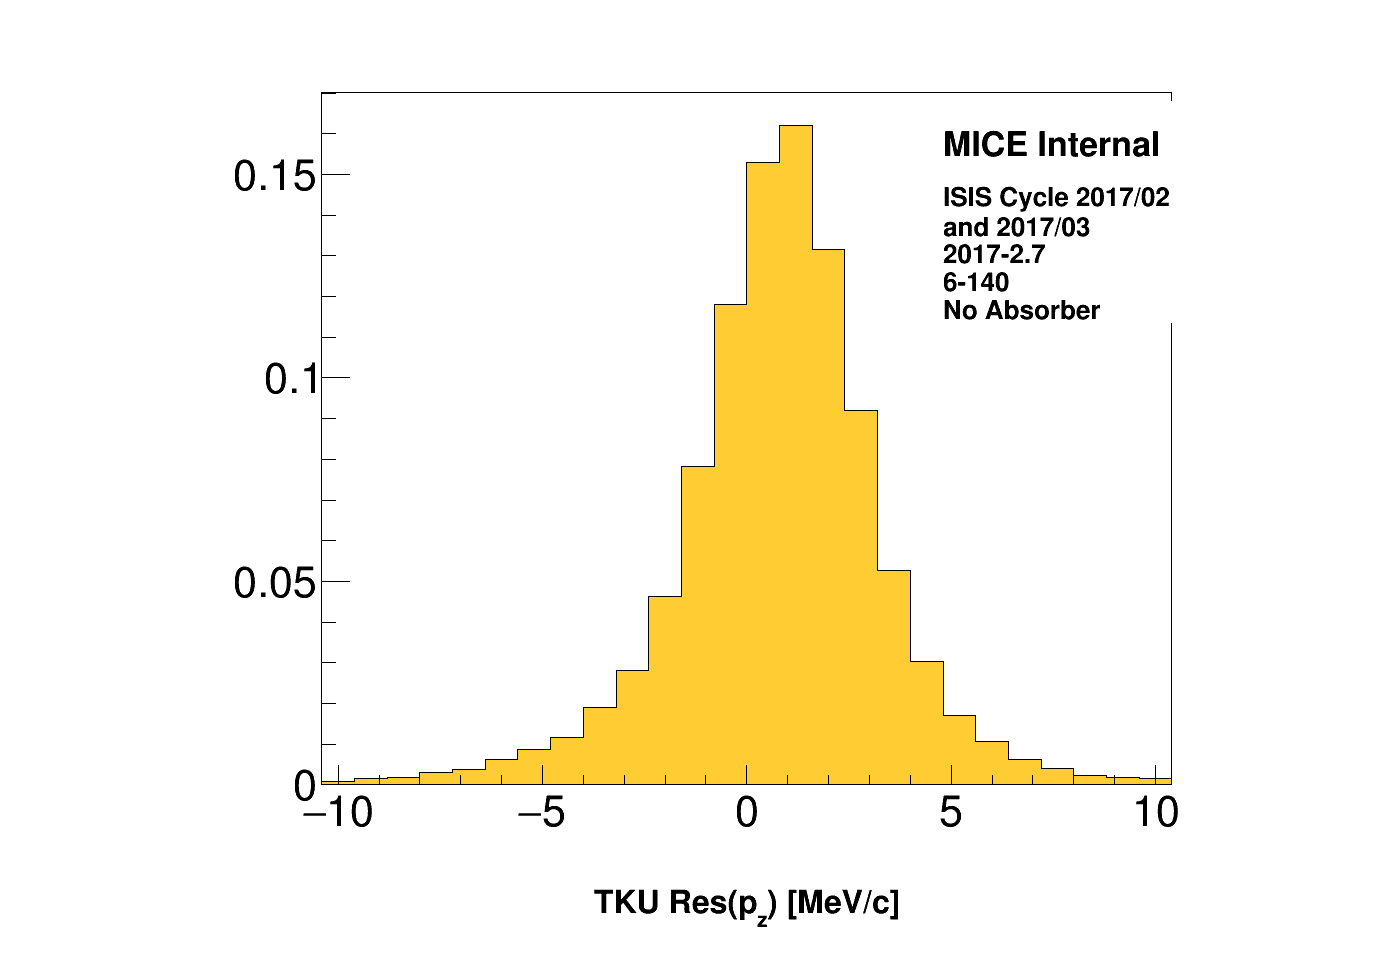
\includegraphics[width=0.5\textwidth]{03-Detectors/Figures/compare_mc/2017-2.7_6-140_None/tku_pz}
    \caption{Simulated TKU resolution in the transverse phase space variables and $pz$ for events in the upstream sample. \label{fig:tku_resolution}}
\end{figure}


\begin{figure}[!tbh]
    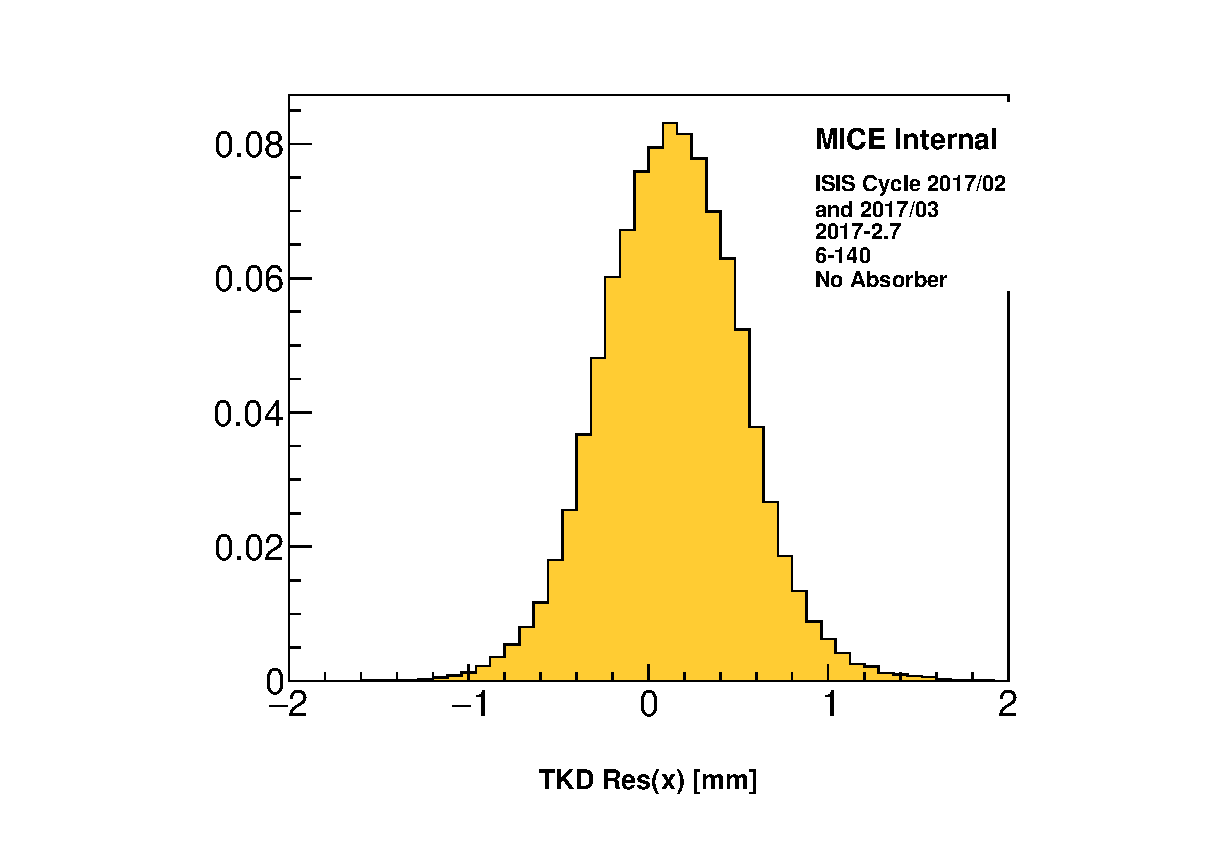
\includegraphics[width=0.5\textwidth]{03-Detectors/Figures/compare_mc/2017-2.7_6-140_None/tkd_x}
    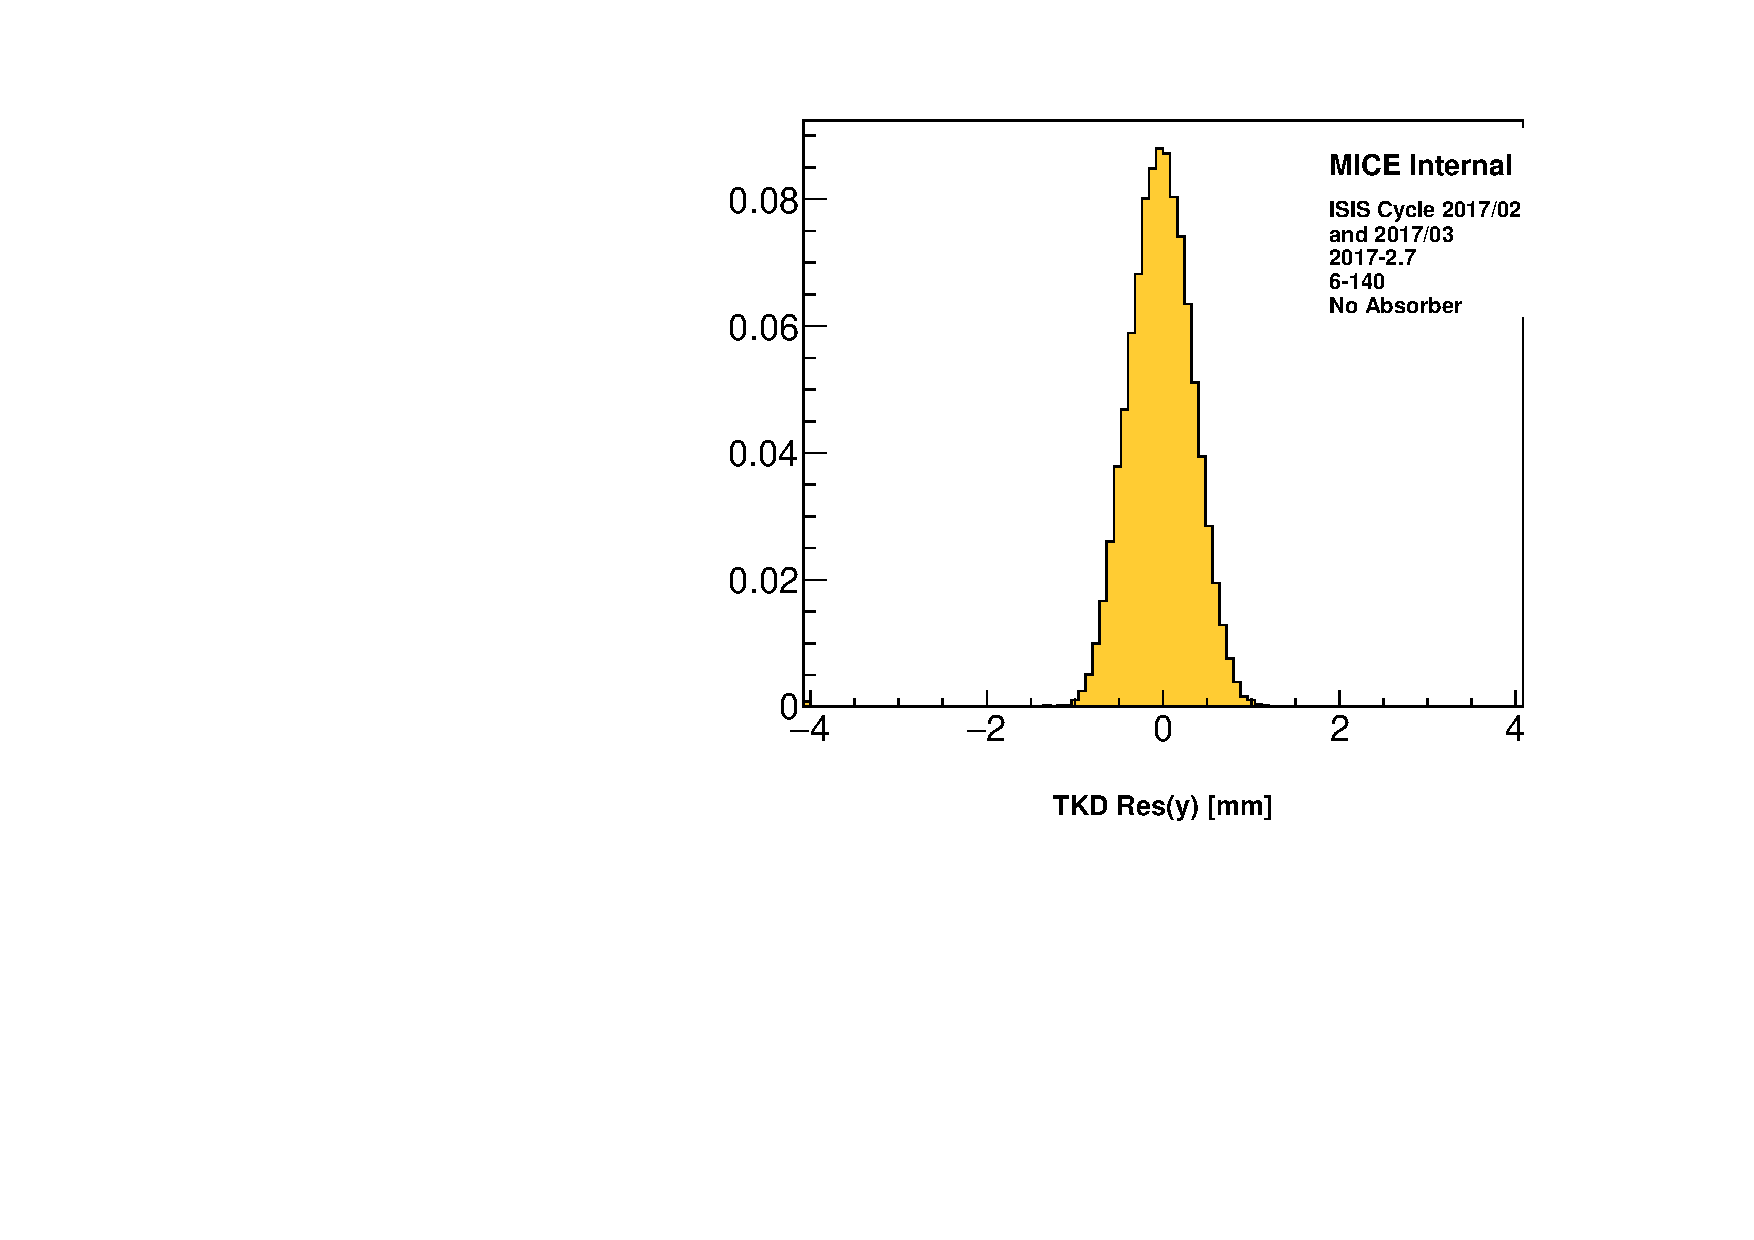
\includegraphics[width=0.5\textwidth]{03-Detectors/Figures/compare_mc/2017-2.7_6-140_None/tkd_y}
    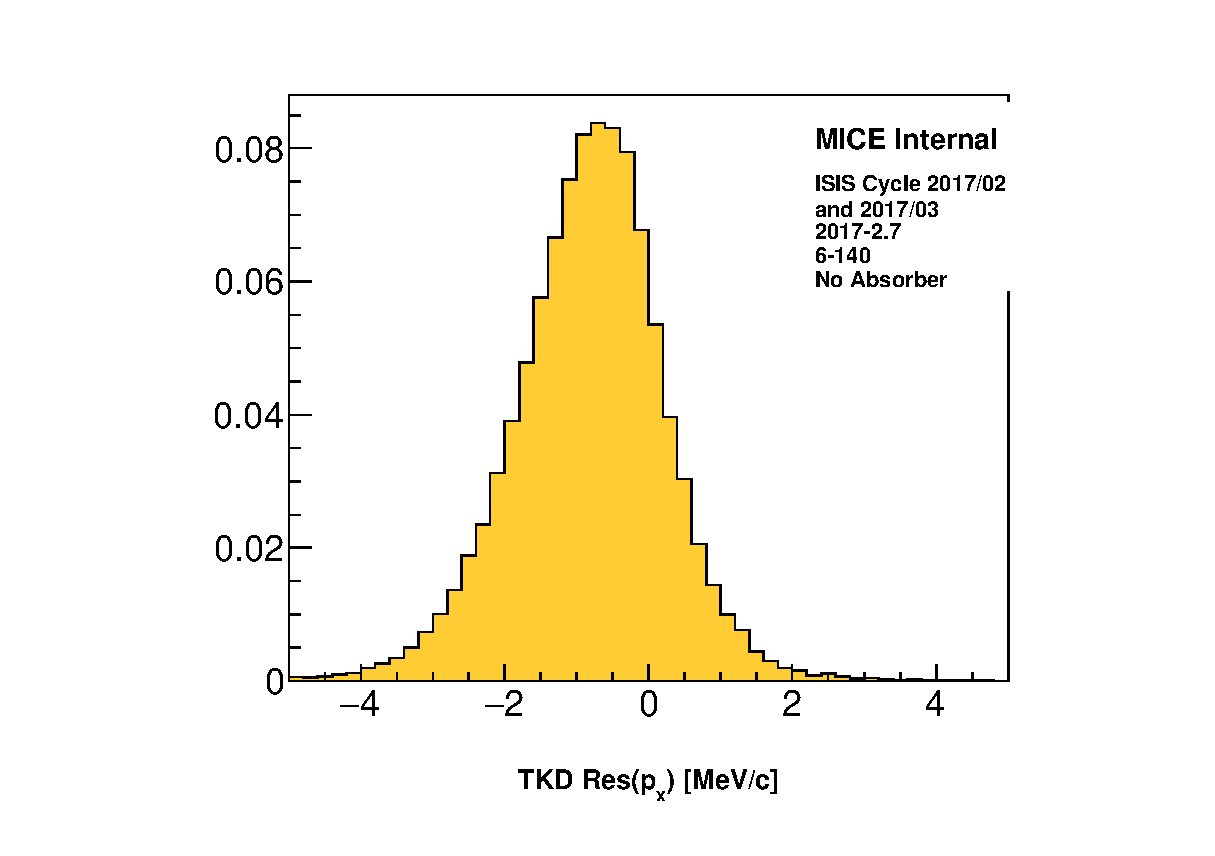
\includegraphics[width=0.5\textwidth]{03-Detectors/Figures/compare_mc/2017-2.7_6-140_None/tkd_px}
    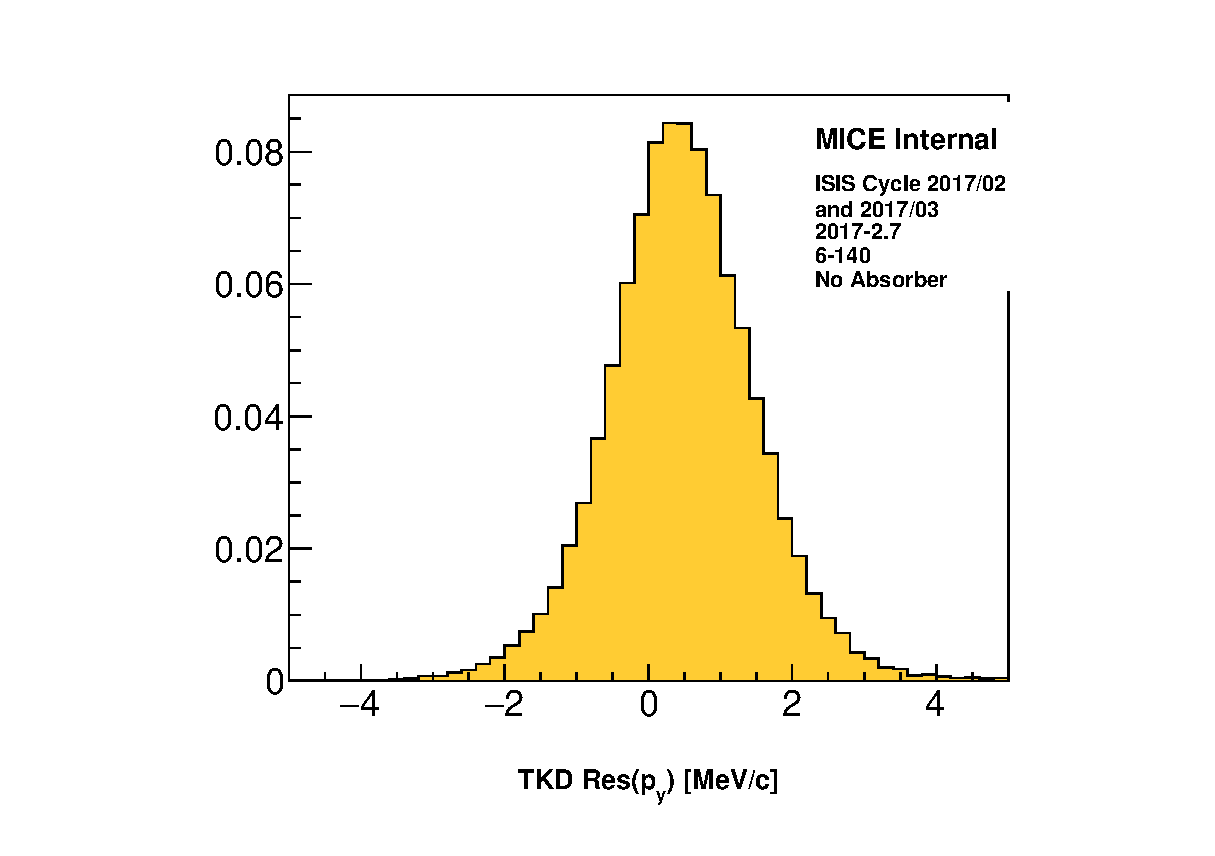
\includegraphics[width=0.5\textwidth]{03-Detectors/Figures/compare_mc/2017-2.7_6-140_None/tkd_py}
    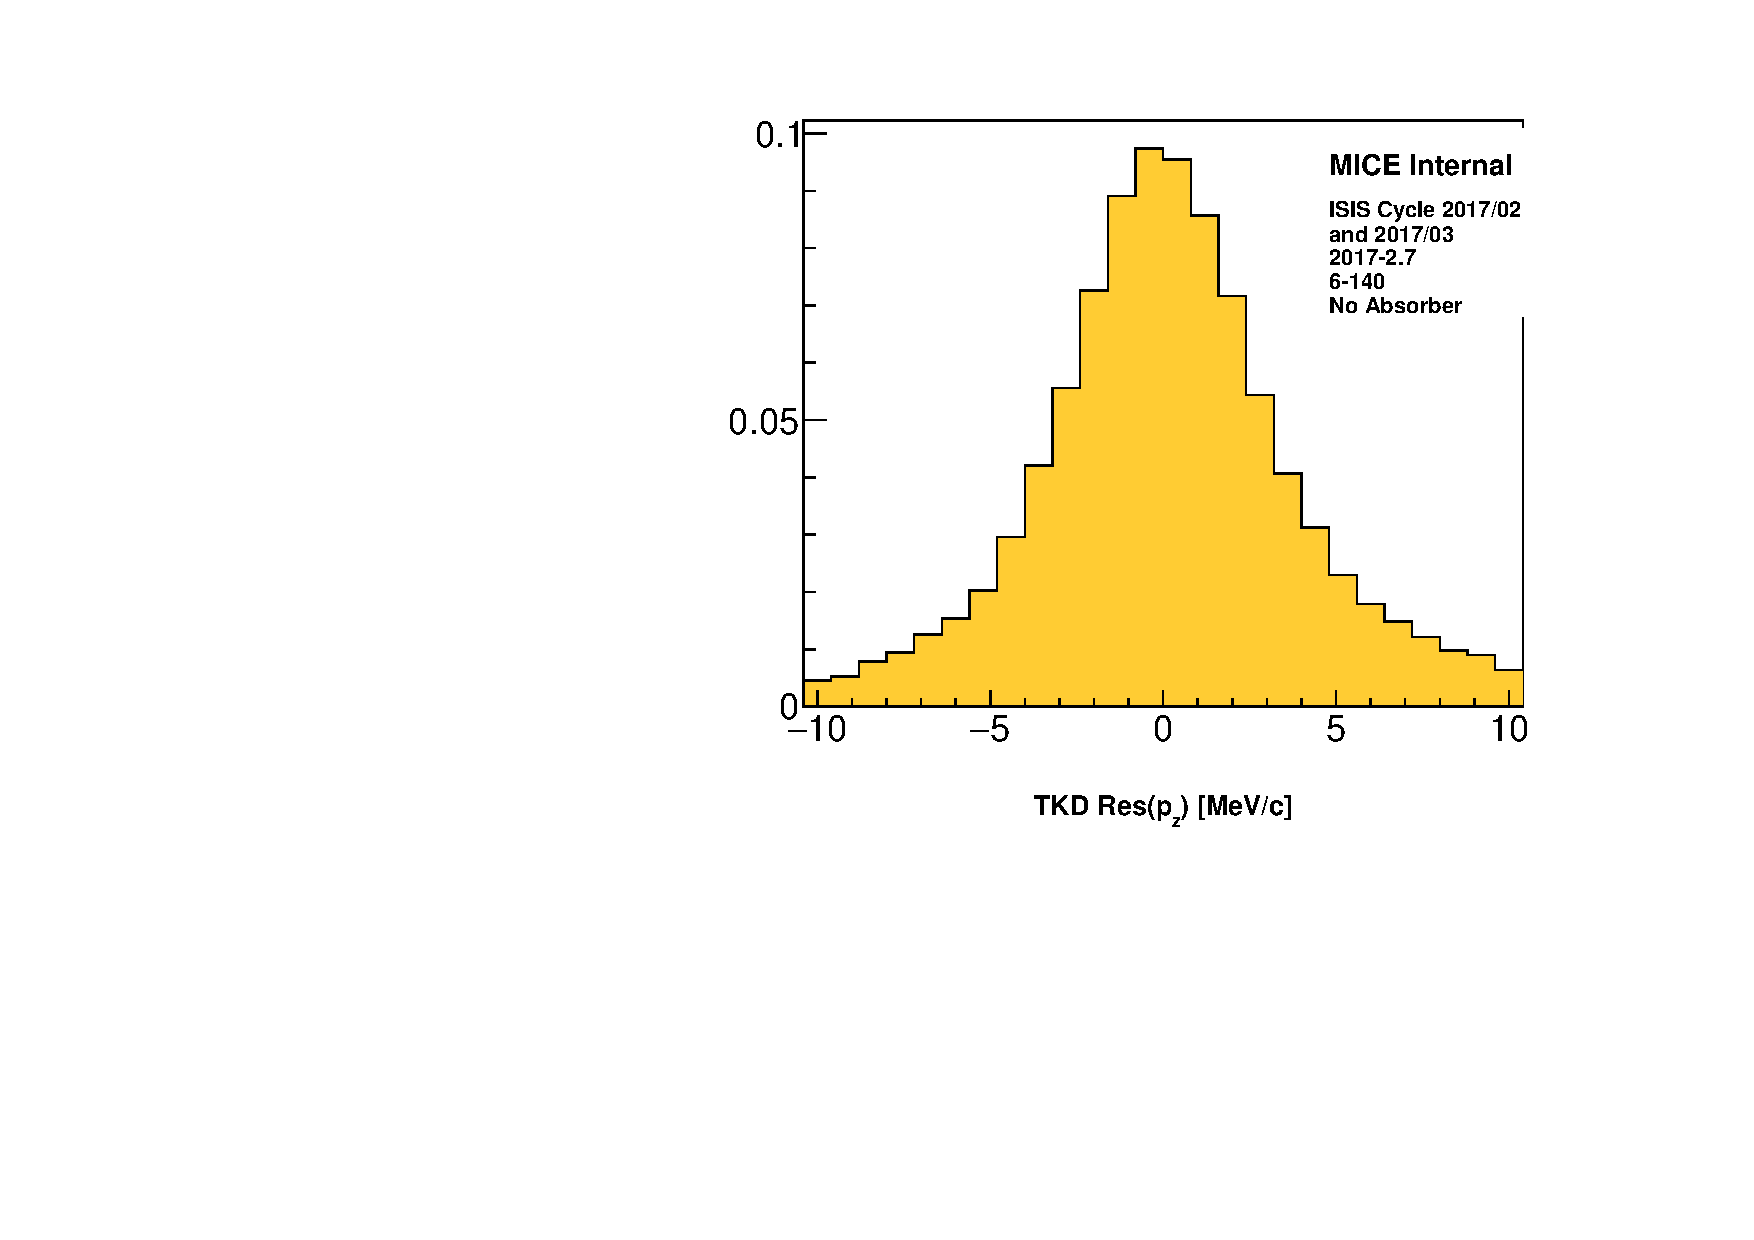
\includegraphics[width=0.5\textwidth]{03-Detectors/Figures/compare_mc/2017-2.7_6-140_None/tkd_pz}
    \caption{Simulated TKD resolution in the transverse phase space variables and $pz$ for events in the downstream sample. \label{fig:tkd_resolution}}
\end{figure}

\subsubsection{Inefficiency and Impurity}

The efficiency of track-finding can be studied. This analysis will
count the change in the number of events in different bins in amplitude. 
Impurity can lead to an overestimation of the number of events in a bin. 
Inefficiency can lead to an underestimation of the number of events in a bin.
Because the sample is defined according to events measured in the upstream
tracker, only inefficiency in the downstream tracker contributes to 
uncertainties in this analysis. Impurity in both trackers can contribute to
uncertainties.

\begin{figure}[!tbh]
    \centering
    \topmatterallplots{02-Cuts}{compare_cuts}{tkd_scifi_n_planes_with_clusters_11_1}
    %tkd_scifi_n_planes_with_clusters_12_1.pdf
    {Number of planes in TKD that contain at least one cluster. Here we 
    take all events in the upstream sample, and add the requirement that exactly 
    one space point was reconstructed in ToF2 and no track was reconstructed in 
    TKD. \label{fig:tkd_inefficient_tracks}}
\end{figure}

The inefficiency can be estimated by studying the response in detectors other 
than the tracker and comparing this with the tracker response. The number of
clusters in events contained within the upstream sample, not making a TKD track
but making exactly one ToF2 space point is shown in fig. 
\ref{fig:tkd_inefficient_tracks}. These tracks are candidates for reconstruction
inefficiency; they may be real particles that did not make a track, for example
due to excess scattering leading to a rejection by the pattern recognition phase 
of the reconstruction.

\begin{figure}[!tbh]
    \centering
    \topmatterallplots{02-Cuts}{compare_cuts}{tku_scifi_n_planes_with_clusters_8_1}
    %tku_scifi_n_planes_with_clusters_9_1.pdf
    {Number of planes in TKU that contain at least one cluster. Here we 
    take all events in the upstream sample, except we require that no TKU track 
    was constructed. The peak around 13-14 planes are real particles in TKU that were 
    not reconstructed. A few events are observed with fewer than 5 clusters which
    may be associated with noise. \label{fig:tku_impure_tracks}}
\end{figure}


\begin{figure}[!tbh]
    \centering
    \topmatterallplots{02-Cuts}{compare_cuts}{tkd_scifi_n_planes_with_clusters_10_1}
    %tkd_scifi_n_planes_with_clusters_11_1.pdf
    {Number of planes in TKD that contain at least one cluster. Here we 
    take all events in the upstream sample, and add the requirement that no 
    track was reconstructed in TKD. The peak at 15 planes are real particles in 
    TKD that were not reconstructed. The peak at 5 planes arises due to noise. 
    In the overlap region, a few events may have sufficient clusters to produce 
    a track, which could lead to impurity due to noise. \label{fig:tkd_impure_tracks}}
\end{figure}

Impurity can arise due to noise in the tracker readout, leading to clusters and 
even tracks that are not associated with a particle. The magnitude can be 
estimated in TKU by studying the number of planes that register at least one 
cluster in events that pass the ToF01 cuts but did not make a TKU track. By 
observing the amount of noise in the tracker, one can infer the number of impure 
tracks. The distribution of noise for these events is shown in fig.
\ref{fig:tku_impure_tracks}. There are a few events with 1 or 2 clusters, but 
there is not enough noise to contribute significantly to track construction. 

The magnitude can be estimated similarly in TKD by studying
the number of clusters in events that pass the upstream cuts but did not make 
a TKD track or a ToF2 space point. These events are expected to correspond to
events where no particle traversed the detector. This is shown in 
\ref{fig:tkd_impure_tracks}. There is a clear separation between the peak 
corresponding to noise events ($<4$ clusters) and the peak corresponding to real 
tracks. 

There is a significant discrepancy between the simulated distribution of 
clusters and the measured distribution of clusters. This is not expected to
effect the simulated inefficiency significantly as the dominant source of 
inefficiency arises due to processes like scattering in the detector planes
deforming the muon helix and causing pattern recognition to fail.

The resultant inefficiency of TKD is shown as a function
of phase space in Fig. \ref{fig:inefficiency_xy_tkd}, \ref{fig:inefficiency_xpx_tkd},
\ref{fig:inefficiency_xpy_tkd} and \ref{fig:inefficiency_pxpy_tkd}, calculated 
using eq \ref{eq:efficiency}. At low $p_t$ track
reconstruction is challenging because scattering in the tracker stations is
dominant over curvature due to the magnetic field. Where this is the case, no
$p_z$ can be reconstructed and the tracks are rejected. Additional inefficiency
is observed at large amplitudes. This may arise due to deformation of the track
helix in the non-uniform fields near to the end coils.

\begin{figure}[!tbh]
    \topmattersysplot{05-Results/Figures/systematics_summary}{140_efficiency}
                     {efficiency_x_vs_y}
            {TKD efficiency as a function of $x$ and $y$ for 3-140 (top left);
             4-140 (top right); 6-140 (bottom left) and 10-140 (bottom right)
             configuratons.
             \label{fig:inefficiency_xy_tkd}}
\end{figure}

\begin{figure}[!tbh]
    \topmattersysplot{05-Results/Figures/systematics_summary}{140_efficiency}
                     {efficiency_x_vs_px}
            {TKD efficiency as a function of $x$ and $p_x$ for 3-140 (top left);
             4-140 (top right); 6-140 (bottom left) and 10-140 (bottom right)
             configuratons.
             \label{fig:inefficiency_xpx_tkd}}
\end{figure}

\begin{figure}[!tbh]
    \topmattersysplot{05-Results/Figures/systematics_summary}{140_efficiency}
                     {efficiency_x_vs_py}
            {TKD efficiency as a function of $x$ and $p_y$ for 3-140 (top left);
             4-140 (top right); 6-140 (bottom left) and 10-140 (bottom right)
             configuratons.
             \label{fig:inefficiency_xpy_tkd}}
\end{figure}

\begin{figure}[!tbh]
    \topmattersysplot{05-Results/Figures/systematics_summary}{140_efficiency}
                     {efficiency_px_vs_py}
            {TKD efficiency as a function of $p_x$ and $p_y$ for 3-140 (top left);
             4-140 (top right); 6-140 (bottom left) and 10-140 (bottom right)
             configuratons.
             \label{fig:inefficiency_pxpy_tkd}}
\end{figure}

\clearpage

\subsection{ToF}

\label{sec:tof_recon}

\begin{figure}[!tbh]
    \centering
    \topmatterallplots{03-Detectors}{compare_data}{tof0_slab_dt}
    {Measured time difference between ToF0 slabs for events in the upstream sample.}
\end{figure}

\begin{figure}[!tbh]
    \centering
    \topmatterallplots{03-Detectors}{compare_data}{tof1_slab_dt}
    {Measured time difference between ToF1 slabs for events in the upstream sample.}
\end{figure}

\begin{figure}[!tbh]
    \centering
    \topmatterallplots{03-Detectors}{compare_data}{tof2_slab_dt}
    {Measured time difference between ToF2 slabs for events in the downstream sample that make a ToF2 space point.}
\end{figure}

Three ToF stations are used to measure the time at which particles pass through
the experiment. The ToF stations consist of two layers aligned at right angles,
each made up of several
scintillating plastic slabs. Each slab has a PMT at either end that records the
time at which particles pass through the detector. Reconstruction software
searches for coincidences of the PMTs at either end of a slab and coincidences
of slabs in each layer in order to make a ToF "space point". A calibration is
applied to account for cable lengths and correct for so-called ``time walk''
that arises due to a different PMT response for a different charge deposited by
the PMT.

The ToF resolutions can be estimated by comparing the reconstructed time 
between each slab, after calibration. This is shown for each of the ToF 
detectors in fig. \ref{fig:tof0_slab_dt}, \ref{fig:tof1_slab_dt} and
\ref{fig:tof2_slab_dt}. Inconsistency in the reconstruction at the 100 ps level
has been observed. Investigation has shown calibration issues that effect the 
calibration differently in different pixels. The resolution is considered 
acceptable for this analysis as the muons are not highly relativistic. The 
inconsistency is greater for the simulation.

As the ToF is only used for validation of the tracker and for particle 
identification in the upstream region, impurity and inefficiency in the ToF does 
not affect this analysis.

\clearpage

\subsection{Global reconstruction}

The overall detector performance can be validated by extrapolating tracks from
one detector to another and comparing the reconstructed coordinates with the 
extrapolated values. Tracks measured in
the upstream tracker are extrapolated upstream to ToF1 and ToF0, and downstream
to TKD and ToF2. Where there are materials in the beamline, the energy change on
passing through the material is estimated using the most probably energy loss. 
Material thicknesses are approximated by the on-axis thickness.  Tracks were
extrapolated through the fields using 4th-order Runge-Kutta integration of the 
Lorentz force law.

Asymmetric effects can be introduced due to scattering from the walls of the
cooling channel as the beam is not symmetric in the channel. In order to 
minimise the effects of such scattering, only events whose projected 
trajectory is  significantly distant from the apertures are considered in this 
analysis. The following sample selection is considered:

\begin{itemize}
\item{Downstream sample:} Events must be included in the downstream sample to
be considered in this analysis
\item{Aperture cut:} The projected upstream track must be within 100 mm radius 
from the beam axis at the following apertures: the upstream absorber safety window;
the upstream absorber window; the absorber centre; the downstream absorber window;
the downstream absorber safety window; the upstream edge of SSD; the Helium window
in SSD; the downstream edge of the downstream PRY aperture. This is performed
even when the lH2 absorber was not installed, for the sake of consistency and
because in some instances mounting flanges can limit the aperture.
\item{1 space point in ToF2:} The event must have exactly one space point in ToF2.
\item{Successful track extrapolation to TKD and ToF2:} The projected upstream track must
have been successfully extrapolated to TKD and ToF2
\end{itemize}

The sample sizes are shown for data in table \ref{tab:data_cuts_summary_2_0} and
\ref{tab:data_cuts_summary_2_1}. The equivalent MC sample sizes are listed in 
\ref{tab:mc_cuts_summary_2_0} and \ref{tab:mc_cuts_summary_2_1}.

\let\splitcell\undefined

\newcommand{\splitcell}[2][c]{%
\begin{tabular}[#1]{@{}c@{}}#2\end{tabular}}


\begin{landscape}
\begin{table}
\centering
\caption{The extrapolated reconstructed data sample is listed.  Samples are listed for 3-140 and 4-140 datasets.\label{tab:data_cuts_summary_2_0}}
\begin{tabular}[pos]{l|cccccccc}
                                                   & \splitcell{\\2017-2.7\\3-140\\None\\} & \splitcell{\\2017-2.7\\3-140\\lH2\\empty\\} & \splitcell{\\2017-2.7\\3-140\\lH2\\full\\} & \splitcell{\\2017-2.7\\3-140\\LiH\\} & \splitcell{\\2017-2.7\\4-140\\None\\} & \splitcell{\\2017-2.7\\4-140\\lH2\\empty\\} & \splitcell{\\2017-2.7\\4-140\\lH2\\full\\} & \splitcell{\\2017-2.7\\4-140\\LiH\\} \\
\hline                                            
Downstream Sample                                  &   12945  &    8598  &    8838  &   11641  &   29028  &   23143  &    8146  &   23345  \\
\hline                                            
Cooling channel aperture cut                       &    7218  &    4735  &    5171  &    6836  &   17681  &   14487  &    4919  &   14254  \\
One space point in ToF2                            &    6954  &    4524  &    4896  &    6485  &   16803  &   13790  &    4597  &   13370  \\
Successful extrapolation to TKD                    &    6954  &    4524  &    4896  &    6485  &   16803  &   13790  &    4597  &   13370  \\
Successful extrapolation to ToF2                   &    6954  &    4524  &    4896  &    6485  &   16803  &   13790  &    4597  &   13370  \\
\hline                                            
Extrapolation Sample                               &    6954  &    4524  &    4896  &    6485  &   16803  &   13790  &    4597  &   13370  \\
\hline                                            

\end{tabular}
\end{table}
\end{landscape}


\begin{landscape}
\begin{table}
\centering
\caption{The extrapolated reconstructed data sample is listed.  Samples are listed for 6-140 and 10-140 datasets.\label{tab:data_cuts_summary_2_1}}
\begin{tabular}[pos]{l|cccccccc}
                                                   & \splitcell{\\2017-2.7\\6-140\\None\\} & \splitcell{\\2017-2.7\\6-140\\lH2\\empty\\} & \splitcell{\\2017-2.7\\6-140\\lH2\\full\\} & \splitcell{\\2017-2.7\\6-140\\LiH\\} & \splitcell{\\2017-2.7\\10-140\\None\\} & \splitcell{\\2017-2.7\\10-140\\lH2\\empty\\} & \splitcell{\\2017-2.7\\10-140\\lH2\\full\\} & \splitcell{\\2017-2.7\\10-140\\LiH\\} \\
\hline                                            
Downstream Sample                                  &   25727  &   16864  &   28459  &   30013  &   12971  &    6430  &   13461  &   15462  \\
\hline                                            
Cooling channel aperture cut                       &   15180  &   10067  &   15993  &   17021  &    5577  &    2796  &    4977  &    5960  \\
One space point in ToF2                            &   14432  &    9478  &   14854  &   15780  &    5257  &    2612  &    4476  &    5373  \\
Successful extrapolation to TKD                    &   14432  &    9478  &   14854  &   15780  &    5257  &    2612  &    4476  &    5373  \\
Successful extrapolation to ToF2                   &   14432  &    9478  &   14854  &   15780  &    5257  &    2612  &    4476  &    5373  \\
\hline                                            
Extrapolation Sample                               &   14432  &    9478  &   14854  &   15780  &    5257  &    2612  &    4476  &    5373  \\
\hline                                            

\end{tabular}
\end{table}
\end{landscape}


\let\splitcell\undefined

\newcommand{\splitcell}[2][c]{%
\begin{tabular}[#1]{@{}c@{}}#2\end{tabular}}


\begin{landscape}
\begin{table}
\centering
\caption{The extrapolated reconstructed simulated sample is listed.  Samples are listed for 3-140 and 4-140 datasets.\label{tab:mc_cuts_summary_2_0}}
\begin{tabular}[pos]{l|cccccccc}
                                                   & \splitcell{\\Simulated\\2017-2.7\\3-140\\None\\} & \splitcell{\\Simulated\\2017-2.7\\3-140\\lH2\\empty\\} & \splitcell{\\Simulated\\2017-2.7\\3-140\\lH2\\full\\} & \splitcell{\\Simulated\\2017-2.7\\3-140\\LiH\\} & \splitcell{\\Simulated\\2017-2.7\\4-140\\None\\} & \splitcell{\\Simulated\\2017-2.7\\4-140\\lH2\\empty\\} & \splitcell{\\Simulated\\2017-2.7\\4-140\\lH2\\full\\} & \splitcell{\\Simulated\\2017-2.7\\4-140\\LiH\\} \\
\hline                                            
Downstream Sample                                  &    8543  &    9103  &    8382  &    8481  &   17915  &    1617  &   18121  &   18111  \\
\hline                                            
Cooling channel aperture cut                       &    5111  &    5218  &    5032  &    5377  &   10864  &     984  &   10754  &   10402  \\
One space point in ToF2                            &    4539  &    4626  &    4499  &    4819  &    9536  &     867  &    9467  &    9117  \\
Successful extrapolation to TKD                    &    4539  &    4626  &    4499  &    4819  &    9536  &     867  &    9467  &    9117  \\
Successful extrapolation to ToF2                   &    4539  &    4626  &    4499  &    4819  &    9536  &     867  &    9467  &    9117  \\
\hline                                            
Extrapolation Sample                               &    4539  &    4626  &    4499  &    4819  &    9536  &     867  &    9467  &    9117  \\
\hline                                            

\end{tabular}
\end{table}
\end{landscape}


\begin{landscape}
\begin{table}
\centering
\caption{The extrapolated reconstructed simulated sample is listed.  Samples are listed for 6-140 and 10-140 datasets.\label{tab:mc_cuts_summary_2_1}}
\begin{tabular}[pos]{l|cccccccc}
                                                   & \splitcell{\\Simulated\\2017-2.7\\6-140\\None\\} & \splitcell{\\Simulated\\2017-2.7\\6-140\\lH2\\empty\\} & \splitcell{\\Simulated\\2017-2.7\\6-140\\lH2\\full\\} & \splitcell{\\Simulated\\2017-2.7\\6-140\\LiH\\} & \splitcell{\\Simulated\\2017-2.7\\10-140\\None\\} & \splitcell{\\Simulated\\2017-2.7\\10-140\\lH2\\empty\\} & \splitcell{\\Simulated\\2017-2.7\\10-140\\lH2\\full\\} & \splitcell{\\Simulated\\2017-2.7\\10-140\\LiH\\} \\
\hline                                            
Downstream Sample                                  &   16809  &    1539  &   17490  &   17549  &    7856  &     667  &    8422  &    8517  \\
\hline                                            
Cooling channel aperture cut                       &   10235  &     895  &    9444  &    9899  &    3392  &     313  &    3221  &    3324  \\
One space point in ToF2                            &    8993  &     783  &    8219  &    8576  &    2927  &     269  &    2772  &    2858  \\
Successful extrapolation to TKD                    &    8993  &     783  &    8219  &    8576  &    2927  &     269  &    2772  &    2858  \\
Successful extrapolation to ToF2                   &    8993  &     783  &    8219  &    8576  &    2927  &     269  &    2772  &    2858  \\
\hline                                            
Extrapolation Sample                               &    8993  &     783  &    8219  &    8576  &    2927  &     269  &    2772  &    2858  \\
\hline                                            

\end{tabular}
\end{table}
\end{landscape}


\let\splitcell\undefined

\begin{figure}[!tbh]
    \centering
    \topmatterallplots{03-Detectors}{compare_globals}{global_through_residual_tof1_x}
    {Residual horizontal (x) position in ToF1 of tracker tracks following extrapolation from TKU. \label{fig:tof1_extrapolated_x}}
\end{figure}

\begin{figure}[!tbh]
    \centering
    \topmatterallplots{03-Detectors}{compare_globals}{global_through_residual_tof1_y}
    {Residual vertical (y) position in ToF1 of tracker tracks following extrapolation from TKU. \label{fig:tof1_extrapolated_y}}
\end{figure}

\begin{figure}[!tbh]
    \centering
    \topmatterallplots{03-Detectors}{compare_globals}{global_through_residual_tof0_t}
    {Residual ToF0 time of the extrapolated track. Track trajectories were drawn from TKU, while the track times were
    drawn from ToF1 with extrapolated offsets for time-of-flight from TKU to ToF1 considered. \label{fig:tof0_extrapolated_t}}
\end{figure}

The extrapolated position following extrapolation to ToF1 is shown in fig.
\ref{fig:tof1_extrapolated_x} and \ref{fig:tof1_extrapolated_y}. In general the width 
of the distributions are comparable between MC and data. Where the diffuser is in
place for higher emittance beams, the extrapolation goes through the diffuser
material so the residuals are wider, owing to the increased scattering from the
diffuser.

The time-of-flight residual in data shows a systematic offset from 0 and relative to the
MC. The offset from 0 gets worse for higher emittance beams. It is thought to be
an intrinsic property of the beam; muons that are scattered in materials between 
the tracker and the ToF have systematically shorter path lengths than the 
extrapolated trajectories, resulting in systematically longer extrapolated time
of flight. There is some level of agreement between data and MC; the deficiency
in the simulated ToF reconstruction as mentioned in sec. \ref{sec:tof_recon} 
is noted and may explain the discrepancy between data and MC here.

\begin{figure}[!tbh]
    \centering
    \topmatterallplots{03-Detectors}{compare_globals}{global_through_residual_tkd_tp_x}
    {Residual $x$ position of TKU tracks extrapolated to TKD, as compared to the tracks in TKD. \label{fig:tkd_extrapolated_x}}
\end{figure}

\begin{figure}[!tbh]
    \centering
    \topmatterallplots{03-Detectors}{compare_globals}{global_through_residual_tkd_tp_y}
    {Residual $y$ position of TKU tracks extrapolated to TKD, as compared to the tracks in TKD. \label{fig:tkd_extrapolated_y}}
\end{figure}

\begin{figure}[!tbh]
    \centering
    \topmatterallplots{03-Detectors}{compare_globals}{global_through_residual_tkd_tp_px}
    {Residual $p_x$ of TKU tracks extrapolated to TKD, as compared to the tracks in TKD. \label{fig:tkd_extrapolated_px}}
\end{figure}

\begin{figure}[!tbh]
    \centering
    \topmatterallplots{03-Detectors}{compare_globals}{global_through_residual_tkd_tp_py}
    {Residual $p_y$ of TKU tracks extrapolated to TKD, as compared to the tracks in TKD. \label{fig:tkd_extrapolated_py}}
\end{figure}

\begin{figure}[!tbh]
    \centering
    \topmatterallplots{03-Detectors}{compare_globals}{global_through_residual_tkd_tp_p}
    {Residual $p_{tot}$ of TKU tracks extrapolated to TKD, as compared to the tracks in TKD. \label{fig:tkd_extrapolated_p}}
\end{figure}

Small misalignments between TKU extrapolated tracks and TKD are observed, 
indicated by the offset of transverse variables from 0, shown in 
fig. \ref{fig:tkd_extrapolated_x} and \ref{fig:tkd_extrapolated_y}. There are known, 
uncorrected misalignments in the detector system and there are expected to be 
additional misalignments in the magnets which could lead to these offsets.

The total momentum shows discrepancy between TKU and TKD of about 1 MeV/c. This
is consistent with the systematic offset in the tracker momentum resolution 
shown in fig. \ref{fig:tku_resolution} and \ref{fig:tkd_resolution}. It is
interesting to note that the level of agreement between MC and data varies
on a setting-by-setting basis in a statistically significant manner. Agreement
is better for the settings where the liquid hydrogen windows were installed.

\begin{figure}[!tbh]
    \centering
    \topmatterallplots{03-Detectors}{compare_globals}{global_through_residual_tof2_t}
    {Residual time of TKU tracks extrapolated to ToF2, as compared to the time measured in ToF2. The track times were
    drawn from ToF1 with appropriate offsets for time-of-flight from TKU to ToF1 considered. \label{fig:tof2_extrapolated_t}}
\end{figure}

\begin{figure}[!tbh]
    \centering
    \topmatterallplots{03-Detectors}{compare_globals}{global_ds_residual_tof2_x}
    {Residual $x$ position of TKD tracks extrapolated to ToF2, as compared to the position measured in ToF2. \label{fig:tof2_extrapolated_x}}
\end{figure}

\begin{figure}[!tbh]
    \centering
    \topmatterallplots{03-Detectors}{compare_globals}{global_ds_residual_tof2_y}
    {Residual $y$ position of TKD tracks extrapolated to ToF2, as compared to the position measured in ToF2. \label{fig:tof2_extrapolated_y}}
\end{figure}

Further small misalignments are observed in the position residuals between ToF2
and tracks extrapolated from TKD. This is attributed to alignment issues.

The discrepancy between the time measured in ToF1 and the time measured in 
ToF2, using the extrapolated TKU track to estimate the time difference, is shown
in fig. \ref{fig:tof2_extrapolated_t}. Discrepancy is observed of the order of
300 ps. Significant discrepancy between MC and data is observed.

The discrepancy between position measured in ToF2 and the extrapolated track
measured in TKD is shown in fig. \ref{fig:tof2_extrapolated_x} and 
\ref{fig:tof2_extrapolated_y}. Discrepancy of the order of 10 mm is observed.
This can arise from misalignment of the detectors in the reconstruction model or
of the magnets.

\subsection{Incorporation into Analysis}
Discrepancies between the measurement and simulation at the level of a few MeV/c
in momentum are observed in both TKU and TKD. These comparisons between the 
various detector systems are the only data-led validations that the 
reconstruction works at all.

The uncertainty is incorporated into the analysis by 
assuming a relatively large uncertainty in the magnetic field in the region of 
TKU and TKD and a significant misalignment. This yields a corresponding 
uncertainty in the absolute momentum scale and reconstructed amplitude 
distributions.

